\chapter{Data Sets}
\label{Chapter data sets}
In order to address our research questions, this thesis considered a group of  data sets from the UCR data archive \cite{UCRArchive2018} and the UEA data archive \cite{bagnall2018uea}.
This Chapter will describe the  data sets that were used to conduct this empirical experiment and their general properties.

\section{UCR/UEA Archives}
\label{DataArchives}
The University of California Riverside (UCR) and the University of East Anglia (UEA) data archives have been used as references in literature for many experiments on time series problems \cite{abanda2019review,fawaz2020inceptiontime,bagnall2017great,yazdanbakhsh2019multivariate,ruiz2020great,fawaz2019deepreview}
and specially for benchmarking the performance of algorithms.

\subsection{UCR Archive}
\label{UCR}
The UCR archive previously had 85 univariate data sets but in 2018 was then expanded to reach 128 data sets.
Despite sharing the property of being univariate, the data sets cover a variety of values for other aspects like;
training data size [16, 8926]; testing data size [20, 16800]; number of classes [2, 60]; length of time series [15, 2844] and for some data sets length of instances vary within the data set;
and the nature of the data being collected. The archive offers a single predefined train/test split for each of the data sets to facilitate reproducability of results.
Finally, the data is z-normalized; to remove offset and scaling. Z-normalization is the transformation of the data to have a mean of zero and one unit of standard deviation.

\subsection{UEA Archive}
\label{UEA}
The other archive we used is the UEA archive for multivariate data sets. Like the UCR archive, was developed and expanded over time.
It started as a small archive of 12 data sets collected by Mustafa Baydogan,
then later on, in 2018, was expanded to reach 30 data sets as a collaboration between researchers of UEA and UCR. The data sets vary in their characteristics;
training data size [12, 30000]; testing data size [15, 20000]; number of classes [2, 39]; length of time series [8, 17984]; number of dimensions [2, 1345] and six different different groups based on their application area.
The archive was processed so that the data instances have equal lengths, instances of missing data points were excluded and a single predefined train/test split is provided.

\subsection{Used Data Sets}
\label{used data sets}
For the scope of our experiment, a total of 84 data sets were selected from both archives to be used within the framework.
There were two main points of interest driving our selection criteria for data sets:
\begin{itemize}
    \item The data was collected from real life scenarios, that implies that the time series data collected was measured from existing subjects.
    \item The data represents a real time series structure behind it and not converted from another data format; like images and videos.
\end{itemize}
Based on the previously mentioned criteria we excluded data sets that belonged to type 'Simulated'; to comply with our first criterion.
For the second criterion, we excluded data sets that belonged to either Image or Motion type.
We have also excluded data sets that contain instances of varying lengths; as we believe that time series data imputation is a whole other topic outside the scope of our thesis.

The remaining collection of data sets still represented a wide variety in terms of data criteria. We present the statistics about the remaining data sets all together in figure \ref{fig:DatasetsMetadata}.
Since the smallest data set (StandWalkJump) and the largest data set (InsectWingbeat) are the same as the UEA archive; training and testing data sizes are the same as previously mentioned ranges in the original archive, [12, 30000] and [15, 20000] respectively;
number of classes covers [2, 52]; length of time series the range is [24, 3000], with Chinatown being the shortest and MotorImagery the longest;
the number of dimensions for multivariate data sets still covered the whole range [2, 1345]; and the remaining 15 types are AUDIO, DEVICE, ECG, EEG, EOG, EPG, HAR, HEMODYNAMICS, MISC, OTHER, SENSOR, SOUND, SPECTRO, SPEECH and Traffic.

\begin{figure}
    \captionsetup{justification=raggedright}
    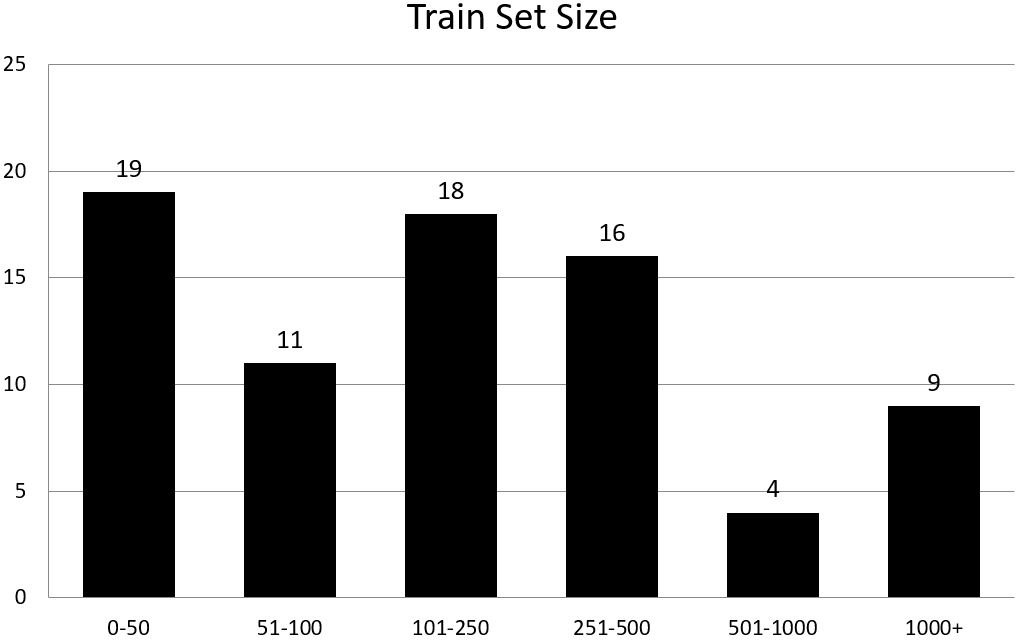
\includegraphics[width=0.49\textwidth,keepaspectratio]{Train_size_hist.JPG}
    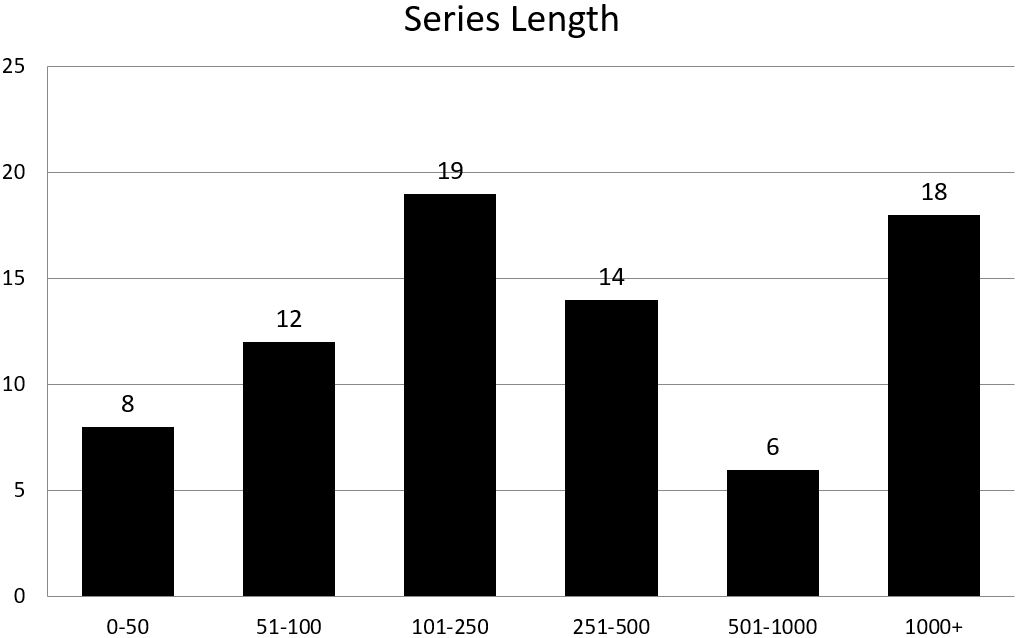
\includegraphics[width=0.49\textwidth,keepaspectratio]{Length_hist.JPG}
    \\[\smallskipamount]
    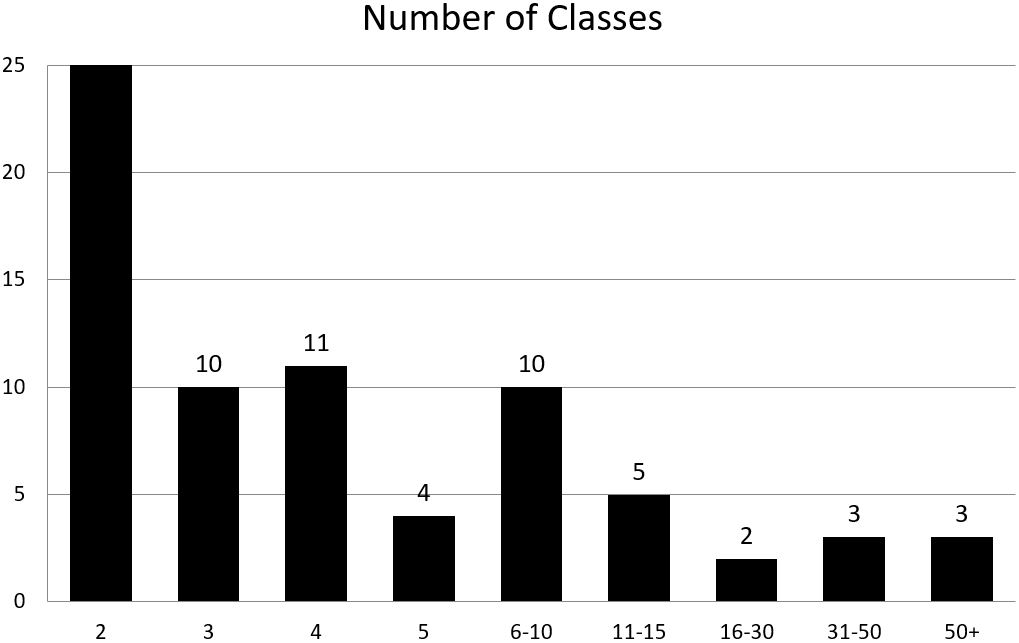
\includegraphics[width=0.49\textwidth,keepaspectratio]{Classes_hist.JPG}
    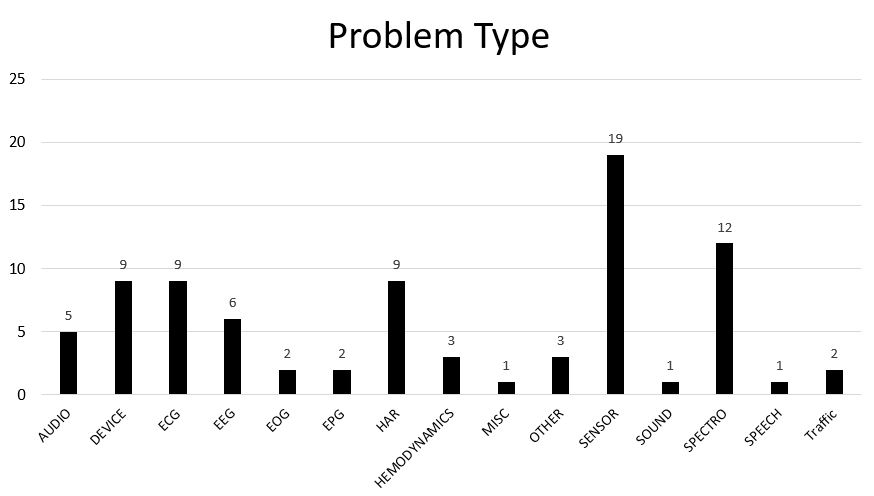
\includegraphics[width=0.49\textwidth,keepaspectratio]{Problem_hist.JPG}
    \caption{Metadata of the used data sets}
    \label{fig:DatasetsMetadata}
\end{figure}

Although the data sets that we used covered a variety of properties, but within some properties there were huge imbalances in the distribution of values.
Within grouping by training data set size, the group of data sets with sizes [501, 1000] was the smallest, with only 4 data sets which is $\frac{1}{3}$ of the next smallest group.
Grouping by series length was the best, among the different groupings, in terms of imbalance. Data sets of lengths [0, 50] were the smallest group with a count of 9 compared to the largest group, length $\geq$ 1001, of 20 data sets.
Number of classes was highly imbalanced; the binary classification group contained 31 data sets, which was more than double the second largest group [6, 10] of 15 data sets.
Finally, there was an over representation of type SENSOR than any other type with a total of 19 data sets.
While multiple other groups were represented by very few data sets like MISC, SOUND and SPEECH which only had 1 data set; or like EOG, EPG and Traffic 2 data sets.

\begin{table}
\begin{center}
 \begin{longtable}{||c|c|c|c|c|c||} 
 
 \hline
  data set & Train & Test & Length & Classes & Type \\ [0.5ex]
 \hline\hline
 ACSF1 & 100 & 100 & 1460 & 10 & DEVICE \\[1ex]
 \hline
 Beef & 30 & 30 & 470 & 5 & SPECTRO \\[1ex]
 \hline
 Car & 60 & 60 & 577 & 4 & SENSOR \\[1ex]
 \hline
 Chinatown & 20 & 345 & 24 & 2 & Traffic \\[1ex]
 \hline
 CinCECGtorso & 40 & 1380 & 1639 & 4 & ECG \\[1ex]
 \hline
 Coffee & 28 & 28 & 286 & 2 & SPECTRO \\[1ex]
 \hline
 Computers & 250 & 250 & 720 & 2 & DEVICE \\[1ex]
 \hline
 DodgerLoopDay & 78 & 80 & 288 & 7 & SENSOR \\[1ex]
 \hline
 DodgerLoopGame & 20 & 138 & 288 & 2 & SENSOR \\[1ex]
 \hline
 DodgerLoopWeekend & 20 & 138 & 288 & 2 & SENSOR \\[1ex]
 \hline
 Earthquakes & 322 & 139 & 512 & 2 & SENSOR \\[1ex]
 \hline
 ECG200 & 100 & 100 & 96 & 2 & ECG \\[1ex]
 \hline
 ECG5000 & 500 & 4500 & 140 & 5 & ECG \\[1ex]
 \hline
 ECGFiveDays & 23 & 861 & 136 & 2 & ECG \\[1ex]
 \hline
 ElectricDevices & 8926 & 7711 & 96 & 7 & DEVICE \\[1ex]
 \hline
 EOGHorizontalSignal & 362 & 362 & 1250 & 12 & EOG \\[1ex]
 \hline
 EOGVerticalSignal & 362 & 362 & 1250 & 12 & EOG \\[1ex]
 \hline
 EthanolLevel & 504 & 500 & 1751 & 4 & SPECTRO \\[1ex]
 \hline
 FordA & 3601 & 1320 & 500 & 2 & SENSOR \\[1ex]
 \hline
 FordB & 3636 & 810 & 500 & 2 & SENSOR \\[1ex]
 \hline
 FreezerRegularTrain & 150 & 2850 & 301 & 2 & SENSOR \\[1ex]
 \hline
 FreezerSmallTrain & 28 & 2850 & 301 & 2 & SENSOR \\[1ex]
 \hline
 Fungi & 18 & 186 & 201 & 18 & OTHER \\[1ex]
 \hline
 Ham & 109 & 105 & 431 & 2 & SPECTRO \\[1ex]
 \hline
 HouseTwenty & 34 & 101 & 3000 & 2 & DEVICE \\[1ex]
 \hline
 InsectEPGRegularTrain & 62 & 249 & 601 & 3 & EPG \\[1ex]
 \hline
 InsectEPGSmallTrain & 17 & 249 & 601 & 3 & EPG \\[1ex]
 \hline
 InsectWingbeatSound & 25000 & 25000 & 600 & 10 & AUDIO \\[1ex]
 \hline
 ItalyPowerDemand & 67 & 1029 & 24 & 2 & SENSOR \\[1ex]
 \hline
 LargeKitchenAppliances & 375 & 375 & 720 & 3 & DEVICE \\[1ex]
 \hline
 Lightning2 & 60 & 61 & 637 & 2 & SENSOR \\[1ex]
 \hline
 Lightning7 & 70 & 73 & 319 & 7 & SENSOR \\[1ex]
 \hline
 Meat & 60 & 60 & 448 & 3 & SPECTRO \\[1ex]
 \hline
 MelbournePedestrian & 1194 & 2439 & 24 & 10 & TRAFFIC \\[1ex]
 \hline
 MoteStrain & 20 & 1252 & 84 & 2 & SENSOR \\[1ex]
 \hline
 NonInvasiveFetalECGThorax1 & 1800 & 1965 & 750 & 42 & ECG \\[1ex]
 \hline
 NonInvasiveFetalECGThorax2 & 1800 & 1965 & 750 & 42 & ECG \\[1ex]
 \hline
 OliveOil & 30 & 30 & 570 & 4 & SPECTRO \\[1ex]
 \hline
 Phoneme & 214 & 1896 & 1024 & 39 & SOUND \\[1ex]
 \hline
 PickupGestureWiimoteZ & 50 & 50 & 0 & 10 & SENSOR \\[1ex]
 \hline
 PigAirwayPressure & 104 & 208 & 2000 & 52 & HEMODYNAMICS \\[1ex]
 \hline
 PigArtPressure & 104 & 208 & 2000 & 52 & HEMODYNAMICS \\[1ex]
 \hline
 PigCVP & 104 & 208 & 2000 & 52 & HEMODYNAMICS \\[1ex]
 \hline
 PLAID & 537 & 537 & 0 & 11 & DEVICE \\[1ex]
 \hline
 Plane & 105 & 105 & 144 & 7 & SENSOR \\[1ex]
 \hline
 PowerCons & 180 & 180 & 144 & 2 & DEVICE \\[1ex]
 \hline
 RefrigerationDevices & 375 & 375 & 720 & 3 & DEVICE \\[1ex]
 \hline
 Rock & 20 & 50 & 2844 & 4 & SPECTRO \\[1ex]
 \hline
 ScreenType & 375 & 375 & 720 & 3 & DEVICE \\[1ex]
 \hline
 SemgHandGenderCh2 & 300 & 600 & 1500 & 2 & SPECTRO \\[1ex]
 \hline
 SemgHandMovementCh2 & 450 & 450 & 1500 & 6 & SPECTRO \\[1ex]
 \hline
 SemgHandSubjectCh2 & 450 & 450 & 1500 & 5 & SPECTRO \\[1ex]
 \hline
 ShakeGestureWiimoteZ & 50 & 50 & 0 & 10 & SENSOR \\[1ex]
 \hline
 SmallKitchenAppliances & 375 & 375 & 720 & 3 & DEVICE \\[1ex]
 \hline
 SonyAIBORobotSurface1 & 20 & 601 & 70 & 2 & SENSOR \\[1ex]
 \hline
 SonyAIBORobotSurface2 & 27 & 953 & 65 & 2 & SENSOR \\[1ex]
 \hline
 StarlightCurves & 1000 & 8236 & 1024 & 3 & SENSOR \\[1ex]
 \hline
 Strawberry & 613 & 370 & 235 & 2 & SPECTRO \\[1ex]
 \hline
 Trace & 100 & 100 & 275 & 4 & SENSOR \\[1ex]
 \hline
 TwoLeadECG & 23 & 1139 & 82 & 2 & ECG \\[1ex]
 \hline
 Wafer & 1000 & 6164 & 152 & 2 & SENSOR \\[1ex]
 \hline
 Wine & 57 & 54 & 234 & 2 & SPECTRO
 \end{longtable}
\end{center}
\caption{List of used Univariate  data sets}
\label{table:Univariate}
\end{table}

\section{Karolinska  data set}
\label{Karolinska}